
\documentclass[supercite]{Experimental_Report}

\title{~~~~~~数据结构实验~~~~~~}
\author{洪炜豪}
\school{计算机科学与技术学院}
\classnum{CS2106}
\stunum{U202115512}
\instructor{周全} % 李平、孙伟平、范晔斌、陈加忠
\date{2022年6月13日}

\usepackage{algorithm, multirow}
\usepackage{algpseudocode}
\usepackage{amsmath}
\usepackage{amsthm}
\usepackage{framed}
\usepackage{mathtools}
\usepackage{subcaption}
\usepackage{xltxtra} %提供了针对XeTeX的改进并且加入了XeTeX的LOGO, 自动调用xunicode宏包(提供Unicode字符宏)
\usepackage{bm}
\usepackage{tikz}
\usepackage{tikzscale}
\usepackage{pgfplots}
\usepackage{listings}
\usepackage{graphicx}
\usepackage{float}
%\usepackage{enumerate}

\pgfplotsset{compat=1.16}

\newcommand{\cfig}[3]{
  \begin{figure}[htb]
    \centering
    \includegraphics[width=#2\textwidth]{images/#1.tikz}
    \caption{#3}
    \label{fig:#1}
  \end{figure}
}

\newcommand{\sfig}[3]{
  \begin{subfigure}[b]{#2\textwidth}
    \includegraphics[width=\textwidth]{images/#1.tikz}
    \caption{#3}
    \label{fig:#1}
  \end{subfigure}
}

\newcommand{\xfig}[3]{
  \begin{figure}[htb]
    \centering
    #3
    \caption{#2}
    \label{fig:#1}
  \end{figure}
}

\newcommand{\rfig}[1]{\autoref{fig:#1}}
\newcommand{\ralg}[1]{\autoref{alg:#1}}
\newcommand{\rthm}[1]{\autoref{thm:#1}}
\newcommand{\rlem}[1]{\autoref{lem:#1}}
\newcommand{\reqn}[1]{\autoref{eqn:#1}}
\newcommand{\rtbl}[1]{\autoref{tbl:#1}}

\algnewcommand\Null{\textsc{null }}
\algnewcommand\algorithmicinput{\textbf{Input:}}
\algnewcommand\Input{\item[\algorithmicinput]}
\algnewcommand\algorithmicoutput{\textbf{Output:}}
\algnewcommand\Output{\item[\algorithmicoutput]}
\algnewcommand\algorithmicbreak{\textbf{break}}
\algnewcommand\Break{\algorithmicbreak}
\algnewcommand\algorithmiccontinue{\textbf{continue}}
\algnewcommand\Continue{\algorithmiccontinue}
\algnewcommand{\LeftCom}[1]{\State $\triangleright$ #1}

\newtheorem{thm}{定理}[section]
\newtheorem{lem}{引理}[section]

\colorlet{shadecolor}{black!15}

\theoremstyle{definition}
\newtheorem{alg}{算法}[section]

\def\thmautorefname~#1\null{定理~#1~\null}
\def\lemautorefname~#1\null{引理~#1~\null}
\def\algautorefname~#1\null{算法~#1~\null}

\begin{document}
\begin{sloppypar}
\maketitle

\clearpage

\pagenumbering{Roman}

\tableofcontents[level=2]
\clearpage

\pagenumbering{arabic}

\section{基于顺序存储结构的线性表实现}

\subsection{问题描述}

线性表是最基本、最简单、也是最常用的一种数据结构。线性表(linear list)是数据结构的一种,一个线性表是n个具有相同特性的数据元素的有限序列。\\

顺序线性表中数据元素之间的关系是一对一的关系,即除了第一个和最后一个数据元素之外,其它数据元素都是首尾相接的。这些数据元素在物理存储中相邻。\\

在数据结构逻辑层次上细分,线性表可分为一般线性表和受限线性表。一般线性表也就是我们通常所说的“线性表”,可以自由的删除或添加结点。受限线性表主要包括栈和队列,受限表示对结点的操作受限制。\\

线性表的逻辑结构简单,便于实现和操作。因此,线性表这种数据结构在实际应用中是广泛采用的一种数据结构。\\

本实验的目的是制作一个一般线性表,并对其能够实现进行一些基本和进阶操作。\\

\subsection{系统设计}

由于顺序线性表的结构简单,使用数组即可轻松对应实现。线性表结构的声明如下:

\begin{lstlisting}[breaklines][breaklines][language=C]

typedef struct{  //顺序表(顺序结构)的定义
	ElemType * elem;
	int length;
	int listsize;
}SqList;

typedef struct{  //线性表的管理表定义
     struct { char name[30];
     		  SqList L;	
      } elem[10];
      int length;
      int listsize;
 }LISTS;
\end{lstlisting}

在系统的执行中,给出系统可执行的功能,先读取用户输入的功能编号,然后利用Switch语句判断来执行对应的功能函数。这种系统结构便于增加和删除功能,代码也更加直观,不易出错。后续实验的系统均沿用此系统结构,不再赘述。

\subsection{系统实现}

1.创建线性表

\begin{lstlisting}[breaklines][language=C]

status InitList(SqList& L)//线性表初始化 
{
	if(L.elem){
        return INFEASTABLE;
	}
	L.elem = (ElemType *)malloc( LIST_INIT_SIZE * sizeof (ElemType)); //分配初始内存
	L.length=0;//设置初始表长
	L.listsize=LIST_INIT_SIZE;//初始化元素容量
	return OK;
}

\end{lstlisting}

2.销毁线性表

\begin{lstlisting}[breaklines][language=C]

status DestroyList(SqList& L)
{
    if(!L.elem){
        return INFEASTABLE;
	}
	free (L.elem);//释放数据元素的空间
	L.elem=NULL;//指针设为空
    L.length=0;//长度置零
    L.listsize=0;
	return OK; 
}

\end{lstlisting}

3.清空线性表

\begin{lstlisting}[breaklines][language=C]

status ClearList(SqList& L)
// 如果线性表L存在,删除线性表L中的所有元素,返回OK,
否则返回INFEASIBLE。
{
    if(!L.elem){
        return INFEASTABLE;
	}
	free (L.elem);
    L.length=0;
    L.listsize=0;
	return OK; 
}

\end{lstlisting}

4.线性表判空

\begin{lstlisting}[breaklines][language=C]

status ListEmpty(SqList L)
// 如果线性表L存在,判断线性表L是否为空,空就返回TRUE,
否则返回FALSE;如果线性表L不存在,返回INFEASIBLE。
{
    if(!L.length&&L.elem){//线性表存在且为空 
        return OK;
    }
    if(L.length&&L.elem){//线性表存在且非空 
        return ERROR;
    }
    if(L.elem==NULL&&L.length==0){//线性表不存在
        return INFEASTABLE;
    }
}

\end{lstlisting}

5.求线性表长度

\begin{lstlisting}[breaklines][language=C]

status ListLength(SqList L)
// 如果线性表L存在,返回线性表L的长度,否则返回INFEASIBLE。
{
    if(L.elem){
        return L.length;
    }
    return INFEASTABLE;
}

\end{lstlisting}

6.获取线性表元素

\begin{lstlisting}[breaklines][language=C]

status GetElem(SqList L,int i,ElemType &e)
// 如果线性表L存在,获取线性表L的第i个元素,保存在e中,返回OK;如果i不合法,返回ERROR;如果线性表L不存在,返回INFEASIBLE。
{
    if(L.elem==NULL){
        return INFEASTABLE;
    }
    if(i<1||i>L.length){
        return ERROR;
    }
     //未执行上方if语句则i合法,获取元素
    e=L.elem[i-1];//逻辑位置转换为物理位置后获取元素保存在e中
    return OK;
}

\end{lstlisting}

7.查找元素

\begin{lstlisting}[breaklines][language=C]

int LocateElem(SqList L,ElemType e)
// 如果线性表L存在,查找元素e在线性表L中的位置序号并返回该序号;如果e不存在,返回0;当线性表L不存在时,返回INFEASIBLE(即-1)。
{
    if(L.elem==NULL){
        return INFEASTABLE;
    }
    int j;
    for(j=0;j<L.listsize;j++){//顺序查找线性表
        if(e==L.elem[j]){ //找到则返回
            return j+1;
        }
    }
    return 0;//遍历一遍没找到返回0
}

\end{lstlisting}

8.查找元素的前驱

\begin{lstlisting}[breaklines][language=C]

status PriorElem(SqList L,ElemType e,ElemType &pre)
// 如果线性表L存在,获取线性表L中元素e的前驱,保存在pre中,返回OK;如果没有前驱,返回ERROR;如果线性表L不存在,返回INFEASIBLE。
{
    if(L.elem==NULL){
        return INFEASTABLE;
    }
    int j;
    for(j=0;j<L.length;j++){
        if(e==L.elem[j])
		{
            if(j!=0){
            pre=L.elem[j-1];
            return OK;
			}
			else{
				return 12;//此处代表存在该元素而该元素在第一个没有前驱
			}
        }
    }
    return ERROR;
}

\end{lstlisting}

9.查找元素的后继

\begin{lstlisting}[breaklines][language=C]

status NextElem(SqList L,ElemType e,ElemType &next)
// 如果线性表L存在,获取线性表L元素e的后继,保存在next中,返回OK;如果没有后继,返回ERROR;如果线性表L不存在,返回INFEASIBLE。
{
    if(L.elem==NULL){
        return INFEASTABLE;
    }
    int j;
    for(j=0;j<L.length;j++){
        if(e==L.elem[j]){
        	if(j!=L.length-1){
        		 next=L.elem[j+1];
            return OK;
			}
           if(j==L.length-1){
           	return 13;  //此处代表存在该元素而该元素在最后一个没有后继
		   }
        }
        
    }
    return ERROR;
}
}

\end{lstlisting}

10.插入元素

\begin{lstlisting}[breaklines][language=C]

status ListInsert(SqList &L,int i,ElemType e)
// 如果线性表L存在,将元素e插入到线性表L的第i个元素之前,返回OK;当插入位置不正确时,返回ERROR;如果线性表L不存在,返回INFEASIBLE。
{
    if(L.elem==NULL){
		printf("线性表不存在!");
        return INFEASTABLE;
    }
    int i;
	if(j==0||j>L.length+1){//如果i超过表长2以上或不为正自然数,则不合法,无法找到对应的插入位置
        return ERROR;
    }
     if(L.length==0){//如果表为空线性表
        L.elem[0]=e;
        L.length++;
        return OK;
    }
    int a[100];
    for(i=0;i<L.length;i++){
        a[i]=L.elem[i];
    }
    L.length++;L.listsize++;
    L.elem=(ElemType *) malloc(sizeof(ElemType)*L.listsize);//扩容线性表
    for(i=j;i<L.length;i++){
        L.elem[i]=a[i-1];
    }
    L.elem[j-1]=e;
    for(i=0;i<j-1;i++){
        L.elem[i]=a[i];
    }
    return OK;
   

\end{lstlisting}

11.删除元素

\begin{lstlisting}[breaklines][language=C]

status ListDelete(SqList &L,int i,ElemType &e)
// 如果线性表L存在,删除线性表L的第i个元素,并保存在e中,返回OK;当删除位置不正确时,返回ERROR;如果线性表L不存在,返回INFEASIBLE。
{
    if(L.elem==NULL){
        return INFEASTABLE;
    }
    int i;
    if(j==0||j>L.length){//如果i超过表长2以上或不为正自然数,则不合法,无法找到对应的删除位置
        return ERROR;
    }
    L.length--;L.listsize--;//表长-1
    e=L.elem[j-1];//保存删除的元素到e
    for(i=j-1;i<L.length;i++){//从删除的位置开始,使其后所有元素向表头移动1
    L.elem[i]=L.elem[i+1];
        }
    return OK;

\end{lstlisting}

12.遍历输出线性表

\begin{lstlisting}[breaklines][language=C]

status ListTraverse(SqList L)
// 如果线性表L存在,依次显示线性表中的元素,每个元素间空一格,返回OK;如果线性表L不存在,返回INFEASIBLE。
{
    if(L.elem==NULL){
        return INFEASTABLE;
    }
    else{
        if(L.length==0){
        L.length++;
        return OK;
    	}
    }
    printf("\n-----------all elements -----------------------\n");
    for(int i=0;i<L.length;i++){
        if(i==0){
            printf("%d",L.elem[i]);
        }
        else{
            printf(" %d",L.elem[i]);
        }
    }
    printf("\n");
    return OK;
}

\end{lstlisting}

附加功能:

13.最大连续子数组和

\begin{lstlisting}[breaklines][language=C]

status MaxSubArray(SqList L)//最大连续子数组和
{
	 if(L.elem==NULL){
        return INFEASTABLE;
    }
    else{
        if(L.length==0){
        L.length++;
        return OK;
    	}
    }
	int thissum=0,maxsum=0,j;
	for(j=0;j<L.length;j++)//只需遍历一遍,算法复杂度O(n) ,当当前累计的值小于0,则归零重新累加 
	{
		thissum+=L.elem[j];
		if(thissum>maxsum)
			maxsum=thissum;
		else if(thissum<0)
			thissum=0;
	}
	return maxsum;
}

\end{lstlisting}

14.和为K的子数组个数 

\begin{lstlisting}[breaklines][language=C]
思想:
暴力求解
从前往后求和sum[i]为到第i项时候的和
那么sum[i:j] = sum[j]-sum[i]
遍历所有区间,用上面的公式快速求出各个区间的值,符合条件则结果+1。

status SubArrayNum(SqList L,int k)//和为K的子数组个数 
{
	if(L.elem==NULL){
        return INFEASTABLE;
    }
    else{
        if(L.length==0){
        L.length++;
        return OK;
    	}
    }
	int sum=0,i,j;
    for (i=0;i<L.length;i++)//对于每个元素,都对其与后面的所有元素进行累加,复杂度O(n^2) 
    {
        int num=0;
        for(j=i;j<L.length;j++){
            num+=L.elem[j];
            if(num==k) sum++;
        }
    }
    return sum;
}

/*哈希表算法
思想:
假如到第i个元素的时候,总和为sum[i],很显然,可以将sum[i]分为两部分:sum[i] = (sum[i]-k)+k,我们在前边已经得到的sum[x],(0<=x<i)中找到能值等于sum[i]-k的那一个,显然x+1到i部分的值就是k,这样的x有几个,那么到当前索引i的时候,就会有几个子数组和为k。

所以做法如下:
遍历nums,并且依次记录累加和sum
使用哈希表d 记录累加和出现的次数 (如果出现过+1,没出现过=1)
查询以当前元素结尾的和为k的子数组有多少个,用sum[i]-k则得到与目标k的差距,找到等于差距的累计和的个数,加到结果上
status SubArrayNum(SqList L,int k)
{
	 Map<Integer,Integer> map=new HashMap<Integer, Integer>();
        map.put(0,1);
        int count=0;
        int sum=0;
        for (int i=0;i<L.length;i++){
            sum+=L.elem[i];
            if (map.get(sum-k)!=null){
                count+=map.get(sum-k);
            }
            //如果总和没出现过,则添加进哈希表,如果出现过,哈希表中的值+1
            if(map.get(sum)==null)
                map.put(sum,1 );
            else
                map.put(sum,map.get(sum)+1 );
        }
        return count;
} 
*/

\end{lstlisting}

15.链表排序

\begin{lstlisting}[breaklines][language=C]

int cmp(const void *a, const void *b){
   ElemType *c=(ElemType*)a; ElemType *d=(ElemType*)b; 
   return *c-*d;
}
status sortList(SqList L)//链表排序
{
	if(L.elem==NULL){
        return INFEASTABLE;
    }
    else{
        if(L.length==0){
        L.length++;
        return OK;
    	}
    }
	qsort(L.elem,L.length,sizeof(L.elem[0]),cmp);//快速排序
	return OK;
}

\end{lstlisting}

16.文件读写
\begin{lstlisting}[breaklines][language=C]
status  SaveList(SqList L,char FileName[])//实现线性表的文件形式保存 
// 如果线性表L存在,将线性表L的的元素写到FileName文件中,返回OK,否则返回INFEASIBLE。
{
    if(L.elem==NULL){
        return INFEASIBLE;
    }
    FILE *fp = fopen(FileName , "w");//定义文件指针
    if (fp == NULL) //只写方式打开文件并判断打开是否成功
	{
	    puts("Fail to open file!");
	    exit(1);
	}
    for(int i=0;i<L.length;i++)  
        fprintf(fp,"%d ",L.elem[i]); 
    fclose(fp);//关闭文件 
    return OK;
}
status  LoadList(SqList &L,char FileName[])
// 如果线性表L不存在,将FileName文件中的数据读入到线性表L中,返回OK,否则返回INFEASIBLE。
{
   
    int i=0;
	if(L.elem){
        return INFEASIBLE;
    }
    FILE* fp = fopen(FileName , "r");
    if (fp == NULL)
	{
	    puts("Fail to open file!");
	    exit(1);
	}
    L.elem=(ElemType *) malloc(sizeof(ElemType)*LIST_INIT_SIZE); //为读取的线性表申请空间
    while(!feof(fp)){
    	fscanf(fp,"%d ",&L.elem[i++]); 
    	L.length++;
	}
    fclose(fp); 
    return OK;
}

\end{lstlisting}

17.多线性表操作

\begin{lstlisting}[breaklines][language=C]

typedef struct{  //线性表的管理表定义
     struct { char name[30];
     		  SqList L;	
      } elem[10];
      int length;
      int listsize;
 }LISTS;
 
void _LISTS()//多线性表操作 
{ 
	LISTS Lists;
    int n,e,op=100;
    char name[30];
    Lists.length=0;
    printf("请输入要创建的顺序表个数\n");
	scanf("%d", &n);
	while(n--)
   {
    	printf("请输入表名\n");
		scanf("%s",name);
   		AddList(Lists,name);
   		printf("输入元素,以回车结束\n");
    	do
  			{
     		scanf("%d",&e); 
			ListInsert(Lists.elem[Lists.length-1].L,Lists.elem[Lists.length-1].L.length+1,e); 
   			}while(getchar()!='\n');
   }
	printf("1.增加新表 2.移除一个线性表 3.查找线性表 4.查看全表 5.对特定表操作 0.返回上级\n");
	printf("输入您的选项\n");
	while(op){
	 	 system("cls");	printf("\n\n");
	 	printf("1.增加新表 2.移除一个线性表 3.查找线性表 4.查看全表 5.对特定表操作 0.返回上级\n");
	 	printf("输入您的选项\n");
	 	scanf("%d",&op);
	 	switch(op){
case 1:
printf("请输入要创建的顺序表个数\n");
scanf("%d", &n);
while(n--)
{
    	printf("请输入表名\n");
	scanf("%s",name);
   	AddList(Lists,name);
   	printf("输入元素,以回车结束\n");
    	do{
     	scanf("%d",&e); 			ListInsert(Lists.elem[Lists.length-1].L,Lists.elem[Lists.length-1].L.length+1,e); 
   		}while(getchar()!='\n');
    getchar();getchar();
	break;
case 2:
	printf("请输入要删除的表名\n");
	scanf("%s",name);
	if (RemoveList(Lists,name)==OK)
	   	{
   			printf("删除成功"); 
		}
   	else printf("删除失败");
   	getchar();getchar();
	break;
case 3:
	printf("请输入要查找的表名\n");
	scanf("%s",name);
	if (n=LocateList(Lists,name))
   	{
   		printf("%s ",Lists.elem[n-1].name);
   		ListTraverse(Lists.elem[n-1].L);
         putchar('\n');
   	}
   	else printf("查找失败");
   	getchar();getchar();
	break;
case 4:
	printflist(Lists);
	getchar();getchar();
	break;
case 5:
	printf("请输入要操作的表名\n");
	scanf("%s",name);
	if (n=LocateList(Lists,name))
   	{
   		__LISTS(Lists,n);//该功能为其中一个线性表做单独操作,进入三级菜单,见附录
   	}
   	else{
   		printf("该表不存在!");
		}
	getchar();getchar();
	break;
case 0:
     break;
    	default:
    	printf("输入有误,请重新输入");
    	getchar();getchar();
    		}	
		}	
  	}
}

status AddList(LISTS &Lists,char ListName[])//创建新表
{
    Lists.elem[Lists.length].L.elem = (ElemType *) malloc(LIST_INIT_SIZE  * sizeof( ElemType ));	
	if ( !Lists.elem[Lists.length].L.elem ){
		printf("存储空间申请失败\n");
		exit(OVERFLOW);
	} 
    Lists.elem[Lists.length].L.length=0;
    Lists.elem[Lists.length].L.listsize=100;
    strcpy(Lists.elem[Lists.length].name,ListName);
    Lists.length++;
}

status RemoveList(LISTS &Lists,char ListName[])
// Lists中删除一个名称为ListName的线性表
{
    int i=0;
    while(Lists.elem[i].name[0]){
        if(!strcmp(Lists.elem[i].name,ListName)){
        	strcpy(Lists.elem[i].name,"0");
            for(int j=i;j<Lists.length-1;j++){
                Lists.elem[j]=Lists.elem[j+1];
            }
            Lists.length--;
            return OK;
        }
        i++;
    }
    return FALSE;
}

int LocateList(LISTS Lists,char ListName[])
// 在Lists中查找一个名称为ListName的线性表,成功返回逻辑序号,否则返回0
{
    int i=0;
    while(Lists.elem[i].name[0]){
        if(!strcmp(Lists.elem[i].name,ListName)){
            return i+1;
        }
        i++;
    }
    return FALSE;
}

void printflist(LISTS Lists)//输出所有的线性表
{
	for(int n=0;n<Lists.length;n++)
   {
   		printf("%s ",Lists.elem[n].name);
   		ListTraverse(Lists.elem[n].L);
        putchar('\n');
   }
}
\end{lstlisting}
\subsection{系统测试}
以下的操作中,线性表的内容为:湖北 1 3 5 湖南 1 1 -2 3 4 -5 6(加入后单独操作) 

\begin{figure}[H]


    \centering
    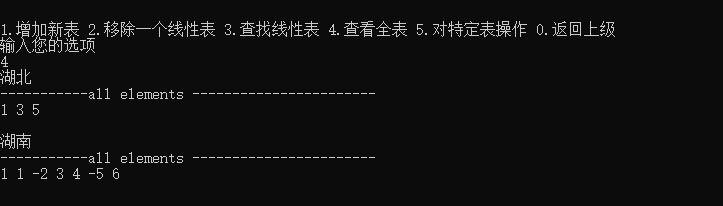
\includegraphics[width=16cm]{pic1//1.png}
    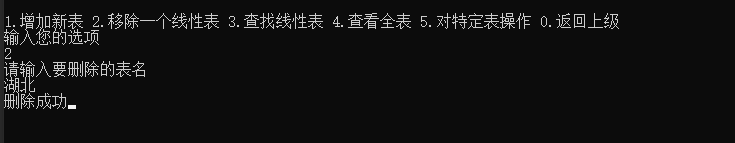
\includegraphics[width=16cm]{pic1//2.png}
    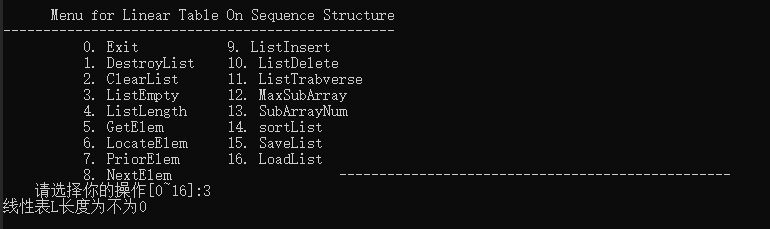
\includegraphics[width=16cm]{pic1//3.png}
    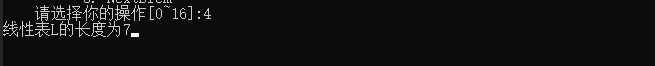
\includegraphics[width=16cm]{pic1//4.png}
	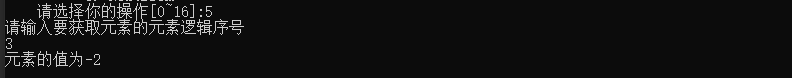
\includegraphics[width=16cm]{pic1//5.png}
	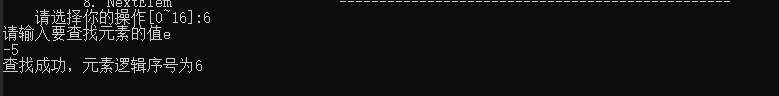
\includegraphics[width=16cm]{pic1//6.png}
	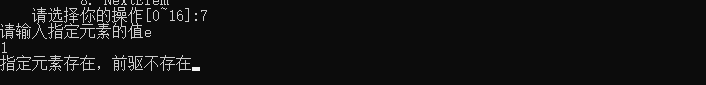
\includegraphics[width=16cm]{pic1//7.png}
	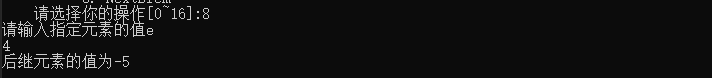
\includegraphics[width=16cm]{pic1//8.png}

\end{figure} 

\begin{figure}[H]
	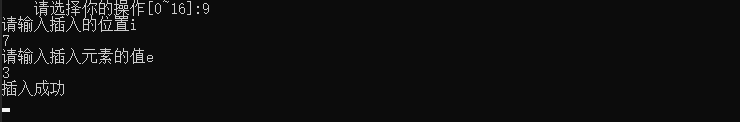
\includegraphics[width=16cm]{pic1//9.png}
	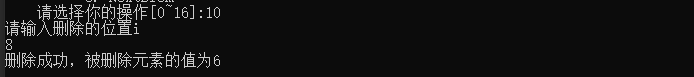
\includegraphics[width=16cm]{pic1//10.png}
	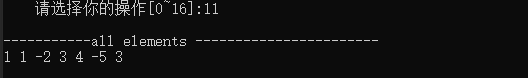
\includegraphics[width=16cm]{pic1//11.png}
	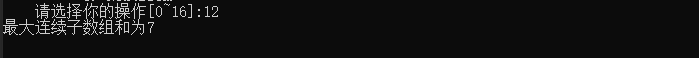
\includegraphics[width=16cm]{pic1//12.png}
	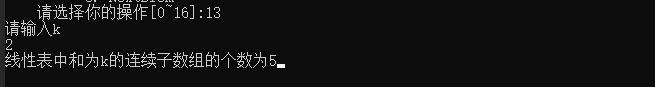
\includegraphics[width=16cm]{pic1//13.png}
	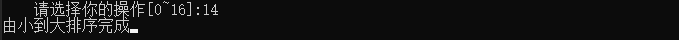
\includegraphics[width=16cm]{pic1//14.png}
	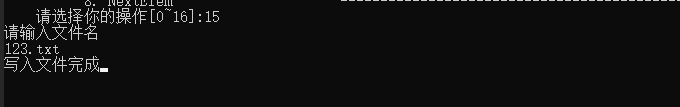
\includegraphics[width=16cm]{pic1//15.png}
	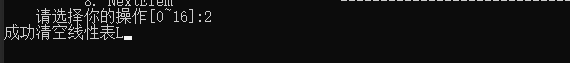
\includegraphics[width=16cm]{pic1//16.png}
	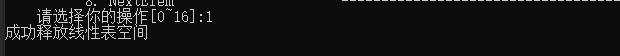
\includegraphics[width=16cm]{pic1//17.png}
	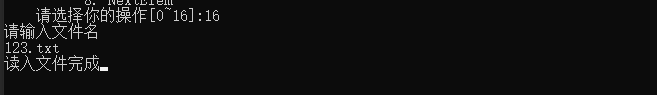
\includegraphics[width=16cm]{pic1//18.png}
	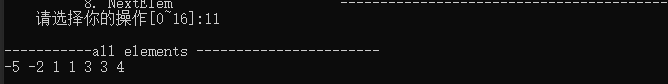
\includegraphics[width=16cm]{pic1//19.png}
\end{figure} 



\subsection{实验小结}
\begin{lstlisting}[breaklines][language=C]
本次实验的重难点有:
1.对函数及其参数的使用,包括\&符号的使用,当使用\&时,会传入参数的地址,能够改变参数本身的值;
2.对顺序线性表结构的熟练理解,确保对线性表执行的操作不产生错误或漏洞;
3.系统结构的设计,对使用进行合理的引导,令用户能够无需学习就上手,方便地使用功能;
4.多个线性表管理表的设计和能够实现对每一个线性表单独操作。
5.细节方面问题的处理:如查找后继元素分为没找到,找到了但是该元素在表尾没有后继,找到该元素且有后继三种情况,都应该说明清楚。

本次实验的心得:
1.顺序线性表的结构简单,便于操作,可以直接用角标对数据元素进行访问,较为直观。
2.顺序线性表的插入和删除操作较为复杂,时间复杂度为O(n)。
3.顺序线性表的前驱和后继可以直接通过下标加减获取,十分便利。
4.对于附加问题,学习了多种算法,
(1)对于连续子数组的最大和,有以下几种方法:
暴力破解:将给定数组的的所有子数组列出来,然后找到子数组和最大的情况,具体来说就是对数组内每一个数A[i]进行遍历,然后遍历以它们为起点的子数组,比较各个子数组的大小,找到最大连续子数组;时间复杂度O(n^2),不应该选择这样的方法。
动态规划:状态方程 : max( dp[ i ] ) = getMax( max( dp[ i -1 ] ) + arr[ i ] ,arr[ i ] )。式子的意义是:从头开始遍历数组,遍历到数组元素 arr[ i ] 时,连续的最大的和 可能为 max( dp[ i -1 ] ) + arr[ i ] ,也可能为 arr[ i ] ,做比较即可得出哪个更大,取最大值。时间复杂度为 n。
一般解法:此为我代码中的解法,对于数组array,从array[1]开始逐个进行相加,与最大值比较,并不停地更替最大值。
(2)对于和为k的子数组个数,有以下几种方法:
暴力破解:对于每个元素,都对其与后面的所有元素进行累加,再比对是否等于k,复杂度O(n^2)。
哈希表: 假如到第i个元素的时候,总和为sum[i],很显然,可以将sum[i]分为两部分:sum[i] = (sum[i]-k)+k,我们在前边已经得到的sum[x],(0<=x<i)中找到能值等于sum[i]-k的那一个,显然x+1到i部分的值就是k,这样的x有几个,那么到当前索引i的时候,就会有几个子数组和为k。
(3)对于链表排序,有以下几种方法:
快速排序:调用c库函数qsort;冒泡排序法;选择排序法等。
\end{lstlisting}

\section{基于链式存储结构的线性表实现}

\subsection{问题描述}

链式线性表具有前一实验中顺序线性表的多数特点,比如其数据元素在逻辑位置上相邻。与其不同的是,链式线性表在物理存储中并不相邻。

链式表分为单链表,循环链表和双向链表。链表可能会设置为空的头结点便于操作,也可能设置尾指针。

本实验的目的是制作一个有空头结点的单链表,并对其能够实现进行一些基本和进阶操作。

\subsection{系统设计}

链式线性表中数据元素的物理位置分开存储,这就要求使用指针来实现。对应每个数据节点,需要增加一个指向下一节点的指针,即指针域,用于串联整个线性表。因此,链式线性表的结构声明如下:

\begin{lstlisting}[breaklines][language=C]

typedef struct LNode{  //单链表(链式结构)结点的定义
      ElemType data;
      struct LNode *next;
    }LNode,*LinkList;
typedef struct LIST{  //多链表的管理表定义
     struct { char name[30];
     		  LinkList L;	
      } elem[10];
      int length;
      int listsize;
 }LISTS;

\end{lstlisting}

\subsection{系统实现}
链表的实现与顺序表具有相似性,此处概不一一举例,仅仅描述附加函数
1.链表翻转
\begin{figure}[H]
	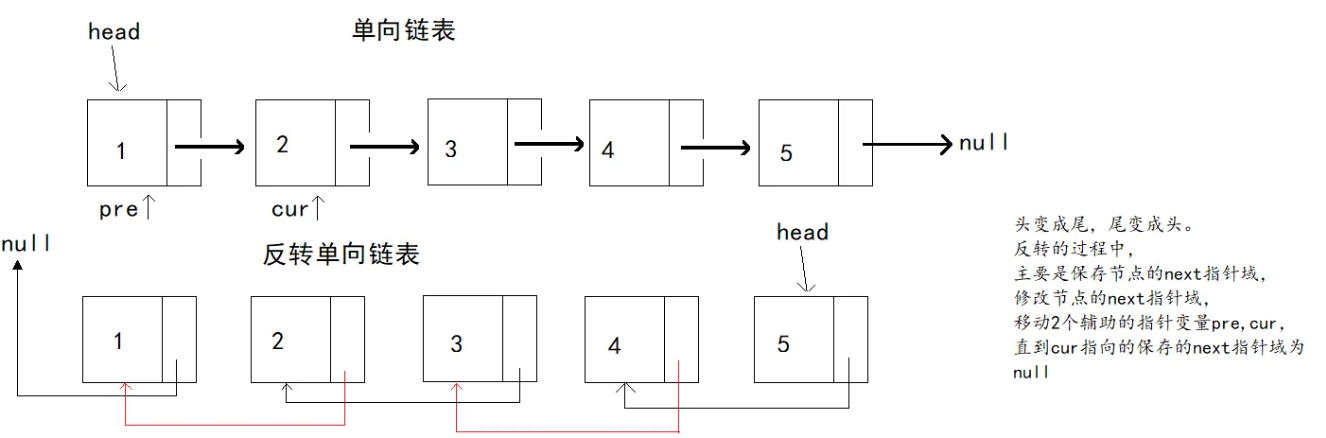
\includegraphics[width=12cm]{pic2//fanzhuan.png}
\end{figure} 
\begin{lstlisting}[breaklines][language=C]
status reverseList(LinkList L)//链表翻转
{
	if(L==NULL){
        return INFEASIBLE;
	}
	LinkList p=L->next,newHead = NULL;
    while (p != NULL) {
        LinkList remain = p->next;
        p->next = newHead;
        newHead = p;
        p = remain;
        }
    L->next=newHead;
    return OK;
}
\end{lstlisting}
2.删除链表的倒数第n个结点(这与删除链表第n个结点几乎相同)
\begin{lstlisting}[breaklines][language=C]

status RemoveNthFromEnd(LinkList L,int n,ElemType &e)//删除链表的倒数第n个结点
{
	if(L==NULL){
        return INFEASIBLE;
	}
	int length=ListLength(L);
	if(n<1||n>length) return ERROR;
	ListDelete(L,length-n+1,e);
	return OK;
}
\end{lstlisting}
3.链表排序(冒泡排序法)
\begin{figure}[H]
	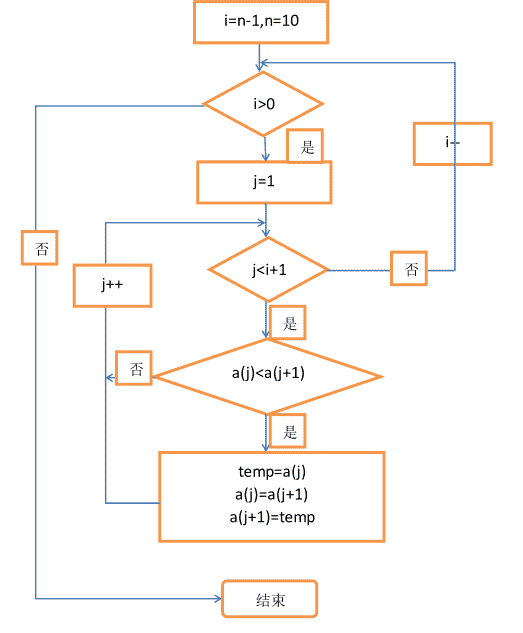
\includegraphics[width=16cm]{pic2//maopao.png}
\end{figure} 
\begin{lstlisting}[breaklines][language=C]

status sortList(LinkList L)//链表排序
{
	if(L==NULL){
        return INFEASIBLE;
	}
	struct LNode *q,*tail;
	int tmp;
	for(tail=NULL;L!=tail;tail=q){
		for(q=L;q->next!=tail;q=q->next){
			if(q->data>q->next->data&&q!=L){
				tmp=q->data;
				q->data=q->next->data;
				q->next->data=tmp;
			}
		}
	}
	return OK;	
}

\end{lstlisting}

4.文件读写

\begin{lstlisting}[breaklines][language=C]

status SaveList(LinkList L,char FileName[])
// 如果线性表L存在,将线性表L的的元素写到FileName文件中,返回OK,否则返回INFEASIBLE。
{
    if(!L){
        return INFEASIBLE;
    }
    FILE *fp;//定义文件指针
    if((fp=fopen(FileName,"w"))==NULL){
    //只写方式打开文件并判断打开是否成功
        exit(-1);
    }
    for(L=L->next;L;L=L->next){
    //顺序遍历,每次写入所访问结点的元素
        fwrite(&L->data,sizeof(ElemType),1,fp);
    }
    fclose(fp);//关闭文件
    return OK;
}

status LoadList(LinkList &L,char FileName[])
// 如果线性表L不存在,将FileName文件中的数据读入到线性表L中,返回OK,否则返回INFEASIBLE。
{
    if(L){
        return INFEASIBLE;
    }
    FILE *fp;//定义文件指针
    if((fp=fopen(FileName,"r"))==NULL){
    //只读方式打开文件并判断打开是否成功
        exit(-1);
    }
    LinkList p;//定义临时指针
    L=(LinkList)malloc(sizeof(LNode));//申请分配结点内存
    p=L;//将头指针值存储在p中
    L->next=NULL;//头结点指针域置空
    ElemType e;//定义临时元素e保存读取的元素值
    while(fread(&e,sizeof(ElemType),1,fp)){
    //一次读取一个元素,直到读取不到元素
        L->next=(LinkList)malloc(sizeof(LNode));//申请分配结点内存
        L=L->next;//L指向新结点,准备对其初始化
        L->data=e;//将读取的元素值放入新结点
        L->next=NULL;//新结点指针域置空
    }
    L=p;//L重新成为头指针
    fclose(fp);//关闭文件
    return OK;
}

\end{lstlisting}

\subsection{系统测试}
略。
\subsection{实验小结}
\begin{lstlisting}[breaklines][language=C]
本次实验的重难点有:
1.对指针的使用,要警惕和避免野指针的出现,容易访问非法内存导致程序出错。例如链表尾结点指针域不为空;
2.对链式线性表结构的熟练理解,确保对线性表执行的操作不产生错误或漏洞。例如结点的插入和删除;
3.链表头结点的使用,不能忽略其存在,也要合理利用其进行便利的数据处理。
4.多个链表管理表的设计和能够实现对每一个链表单独操作。
5.细节方面问题的处理:如查找后继元素分为没找到,找到了但是该元素在表尾没有后继,找到该元素且有后继三种情况,都应该说明清楚。
本次实验的心得:
1.链式线性表的结构虽然也较为简单,便于操作,但相对于顺序线性表复杂,需要思维的转变和习惯。它也失去了顺序表通过角标随机访问的功能。
2.链式线性表的插入和删除操作相对于顺序线性表简单,仅需对目标结点的相邻几个结点进行操作。
3.链式线性表的前驱和后继相对于顺序线性表较为复杂。
4.没有头结点时,链式线性表的前驱获取,以及插入和删除操作需要特判,故增加头结点有很多便利。
5.在进行链表排序时,掌握了冒泡排序法交换数据域和交换指针域两种方法。
交换数据域:冒泡排序,每次从第一个结点开始遍历,比较相邻两个结点的数据域。一趟下来,最大的数据域被交换到最后一个结点。接下来还从头结点起,至倒数第二个结点之间进行冒泡法排序,第二大的被交换到倒数第二个结点,每趟冒泡法排序后,尾部有序的结点增多,这些结点不需要参与下一趟冒泡排序,因此设置一个尾指针tail,它始终指向未排序结点的尾部,排序过程中指针都是和tail比较,判断是否结束循环。
交换指针域:思路与交换数据域相同,不过在成员结果较多时效率较高。
还有一种思路是先把链表的内容存放到数组中(时间为O(n)),然后,我们在对那个数组进行排序(最快为nlog(n)),最后,存放链表中(时间为O(n))。通过计算,我们可以得到它的时间复杂度为(O(nlogn))。
 
\end{lstlisting}
\begin{figure}[H]
	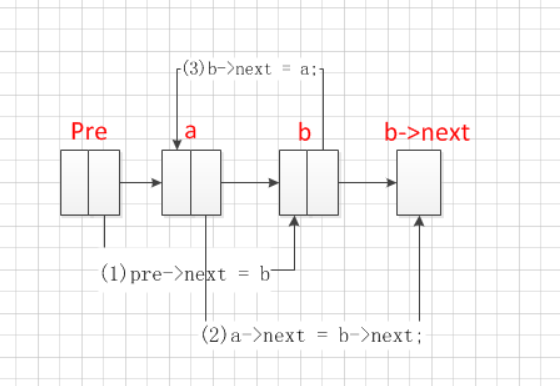
\includegraphics[width=16cm]{pic2//xianglin.png}
\end{figure}
交换指针域图示
\section{基于二叉链表的二叉树实现}

\subsection{问题描述}

二叉树(binary tree)是指树中节点的度不大于2的有序树,它是一种最简单且最重要的树。二叉树的递归定义为:二叉树是一棵空树,或者是一棵由一个根节点和两棵互不相交的,分别称作根的左子树和右子树组成的非空树;左子树和右子树又同样都是二叉树。\\
二叉树(Binary tree)是树形结构的一个重要类型。许多实际问题抽象出来的数据结构往往是二叉树形式,即使是一般的树也能简单地转换为二叉树,而且二叉树的存储结构及其算法都较为简单,因此二叉树显得特别重要。二叉树特点是每个节点最多只能有两棵子树,且有左右之分。\\
二叉树是n个有限元素的集合,该集合或者为空、或者由一个称为根(root)的元素及两个不相交的、被分别称为左子树和右子树的二叉树组成,是有序树。当集合为空时,称该二叉树为空二叉树。在二叉树中,一个元素也称作一个节点。\\
1.节点:包含一个数据元素及若干指向子树分支的信息\\
2.节点的度:一个节点拥有子树的数目称为节点的度\\
3.叶子节点:也称为终端节点,没有子树的节点或者度为零的节点\\
4.分支节点:也称为非终端节点,度不为零的节点称为非终端节点\\
5.树的度:树中所有节点的度的最大值\\
6.节点的层次:从根节点开始,假设根节点为第1层,根节点的子节点为第2层,依此类推,如果某一个节点位于第L层,则其子节点位于第L+1层\\
7.树的深度:也称为树的高度,树中所有节点的层次最大值称为树的深度\\
8.有序树:如果树中各棵子树的次序是有先后次序,则称该树为有序树\\
9.无序树:如果树中各棵子树的次序没有先后次序,则称该树为无序树\\
10.森林:由m(m≥0)棵互不相交的树构成一片森林。如果把一棵非空的树的根节点删除,则该树就变成了一片森林,森林中的树由原来根节点的各棵子树构成

\subsection{系统设计}

二叉树既可以用顺序表按层存储,也可以用二叉链表存储。本次实验中,将二叉树用二叉链表实现。将每个节点设置两个指针域,分别指向其左右孩子,即可将每个节点连接起来。最后给出根节点的指针。

\begin{lstlisting}[breaklines][language=C]

typedef struct {
         KeyType  key;
         char others[20];
	} TElemType; //二叉树结点类型定义

typedef struct BiTNode{  //二叉链表结点的定义
	      TElemType  data;
	      struct BiTNode *lchild,*rchild;
	} BiTNode, *BiTree;

typedef struct moretrees{  //多二叉树的管理表定义
     struct { char name[30];
     		  BiTree T;	
      } elem[10];
      int length;
 }BiTrees;

int front=0,rear=0;
//入队函数
void EnQueue(BiTree *a,BiTree node){
    a[rear++]=node;
}
//出队函数
BiTNode* DeQueue(BiTNode** a){
    return a[front++];
}
\end{lstlisting}

\subsection{系统实现}
0.节点访问函数,用于访问节点操作
\begin{lstlisting}[breaklines][language=C]
void visit(BiTree T)
{
    printf(" %d,%s",T->data.key,T->data.others);
}
\end{lstlisting}

1.创建二叉树

definition的输入规则:\\
二叉树带空子树的先序遍历结点序列,每个结点对应一个整型的关键字和一个字符串,当关键字为0时,表示空子树,为-1表示输入结束

\begin{lstlisting}[breaklines][language=C]


status CreateBiTree(BiTree& T, TElemType definition[],int &i)
/*根据带空枝的二叉树先根遍历序列definition构造一棵二叉树,将根节点指针赋值给T并返回OK,如果有相同的关键字,返回ERROR。*/
{
	/********** Begin *********/
	BiTree ans;
	ans = (BiTree)malloc(sizeof(BiTNode));
	T = ans;
	memset(num, 0, 1000);//num全部置0
	if (definition[0].key == 0|| definition[0].key == -1) {
		T = NULL;
		return OK;
	}//根结点为空的空二叉树
	i = 0;
	if (num[definition[i].key] == 1) return ERROR;//关键字重复
	T = (BiTree)malloc(sizeof(BiTNode));//申请节点内存
	T->data.key = definition[i].key;//数据元素赋值
	strcpy(T->data.others, definition[i].others);//数据元素赋值
	num[definition[i].key] = 1;//表示该key值已经存在,便于查重
	i++;
	if (ERROR == CreateBiTNode(T->lchild, definition, num, i) || ERROR == CreateBiTNode(T->rchild, definition, num, i))
		return ERROR;
	return OK;
	/********** End **********/
}

status CreateBiTNode(BiTree& T, TElemType definition[], int num[], int& i) {
通过递归,将definition[i]之后的数据创建为树节点
	if (definition[i].key == 0 || definition[i].key == -1) {//当前输入是结束语句或空结点,递归终止
		T = NULL;//此分支的指针域置空,代表没有孩子
		i += definition[i].key + 1;//节点计数+1
		return OK;
	}
	if (num[definition[i].key] == 1) return ERROR;//关键字重复
	T = (BiTree)malloc(sizeof(BiTNode));//申请节点内存
	T->data.key = definition[i].key;//数据元素赋值
	strcpy(T->data.others, definition[i].others);//数据元素赋值
	num[definition[i].key] = 1;
	i++;//节点计数+1
	if (ERROR == CreateBiTNode(T->lchild, definition, num, i) || ERROR == CreateBiTNode(T->rchild, definition, num, i))//创建此节点的左、右子树
		return ERROR;
	return OK;
}




\end{lstlisting}

2.销毁二叉树


\begin{lstlisting}[breaklines][language=C]
status DestroyBiTree(BiTree &T)
{
   if(!T){
			 printf("二叉树不存在!\n");
			 getchar();getchar();
			 break;
		 }   
   if (T)
   {
        DestroyBiTree(T->lchild);
        DestroyBiTree(T->rchild);
        free(T);
        T=NULL;
   }
   return OK;
}
\end{lstlisting}

3.清空二叉树

此处递归结构的构建思路是:清空一个子树,就要先清空它的左右子树,递归终止条件是一个节点没有孩子。
\begin{lstlisting}[breaklines][language=C]
status ClearBiTree(BiTree &T)
//将二叉树设置成空,并删除所有结点,释放结点空间
{
    if(!T){
			 printf("二叉树不存在!\n");
			 getchar();getchar();
			 break;
		 }    
    if(T)
    {
        ClearBiTree(T->lchild);
        ClearBiTree(T->rchild);
        free(T);
    }
    T=NULL;
    return OK;
}
\end{lstlisting}

4.二叉树判空

\begin{lstlisting}[breaklines][language=C]

status BiTreeEmpty(BiTree T)
{    
    if(T)
        return FALSE;
    else
        return TRUE;
}

\end{lstlisting}
5.二叉树深度

此处递归结构的构建思路是:求一个子树的深度,就要先求出它的左右子树的深度,取其较大者并+1,递归终止条件是一个节点是空节点,令其返回0。

\begin{lstlisting}[breaklines][language=C]

int max(int a,int b)
{
    if(a>b) return a;
    else return b;
}
int BiTreeDepth(BiTree T)
//通过递归求二叉树T的深度
{ 
    if(T==NULL) return 0; 
    else{
         return 1 + max(BiTreeDepth(T->lchild),BiTreeDepth(T->rchild));
    }
}

\end{lstlisting}

6.查找节点

此处递归结构的构建思路是:令每层递归函数返回一个指针,未查找到则返回空指针,节点对于左右节点的返回值取不为空的指针,即可最终获得查找节点的指针。

\begin{lstlisting}[breaklines][language=C]

BiTNode* LocateNode(BiTree root,KeyType value)
//查找结点
{
    if(root == NULL){
			return NULL;
		}
    else if(root != NULL && root->data.key ==value ){
			return root;
		}
    else{
			BiTree no1 = LocateNode(root->lchild,value);
			BiTree no2 = LocateNode(root->rchild,value);
			if(no1 != NULL && no1->data.key==value){
				return no1;
			}else if(no2 != NULL && no2->data.key==value){
				return no2;
			}
            else{
				return NULL ;
			}
		}
}

\end{lstlisting}

7.节点赋值

\begin{lstlisting}[breaklines][language=C]

void LocateNode1(BiTree T,KeyType e,int &i)
//检查如果进行操作,操作后是否有相同关键字
{
    if(T==NULL) return ;
    if(e==T->data.key){
        i++;//检测到相同关键字,i加1
    }
    LocateNode1(T->lchild,e,i);
    LocateNode1(T->rchild,e,i);
}

status Assign(BiTree &T,KeyType e,TElemType value)
//实现结点赋值。
{
    BiTree q;
    int i=0;//首次执行函数时进行关键字检查
	TElemType j;
    q=LocateNode(T,e);
    if(q==NULL) return ERROR;
    else {
		j=q->data;
        q->data=value;
    }//先进行赋值
    LocateNode1(T,value.key,i);//然后遍历树检查
    if(i<=1) return OK;//如果结点不重复则好赋值成功
    else{
		q->data=j;
		return 13;//如果重复则复原树,返回特定含义
	}
}

\end{lstlisting}

8.获取兄弟节点

\begin{lstlisting}[breaklines][language=C]

BiTNode* Parent(BiTree T,BiTree p)
{/*根据已知节点求父节点的核心代码*/
    if(T==NULL||T==p||p==NULL){/*T==p说明p是根节点,所有没有父节点*/
    	return NULL;
	}
	if(T->lchild==p||T->rchild==p){/*在递归过程中除根节点以外的所有节点总会先被这句代码检查一次,所以T==P只会在根节点处可能被成功触发*/
		return T;
	}
	BiTree temp;
	temp=Parent(T->lchild,p);
	if(temp!=NULL){
		return temp;
	}else{
		return Parent(T->rchild,p);
	}
}

BiTNode* GetSibling(BiTree T,KeyType e)
//实现获得兄弟结点
{
    if(T->data.key==e) return NULL;//树结点无兄弟结点
	BiTree q=LocateNode(T,e);
	BiTree T1=Parent(T,q);//找到父节点
    if(T1->lchild==q){
        return T1->rchild;
    }
   if(T1->rchild==q){
        return T1->lchild;
    }
	return NULL;
}


\end{lstlisting}

9.插入元素

\begin{lstlisting}[breaklines][language=C]

void LocateNode1(BiTree T,KeyType e,int &i)
//检查如果进行操作,操作后是否有相同关键字
{
    if(T==NULL) return ;
    if(e==T->data.key){
        i++;//检测到相同关键字,i加1
    }
    LocateNode1(T->lchild,e,i);
    LocateNode1(T->rchild,e,i);
}
status InsertNode(BiTree &T,KeyType e,int LR,TElemType c)
//插入结点,将元素为c的节点根据LR值插入关键字为e的节点的左或右孩子,LR为-1时,作为根节点插入
{
    LocateNode1(T,c.key,i);
    if(!LocateNode(T,e)){//没找到
        return ERROR;
    }
	if(i) return 13;//若插入,则存在重复元素
    if(LR==-1){//作为根节点插入的情况
        BiTree q = (BiTree)malloc(sizeof(BiTNode));
        q->lchild=NULL;
        q->rchild=T;
        q->data=c;
        T=q;
        return OK;
    }
    else{
        BiTree p=LocateNode(T,e);
        BiTree p1 = (BiTree)malloc(sizeof(BiTNode));
        p1->data=c;
        if(LR==0){//作为左子树插入,原子树作为新节点的右子树
            p1->rchild=p->lchild;
            p1->lchild=NULL;
            p->lchild=p1;
            return OK;
        }
        if(LR==1){//作为右子树插入,原子树作为新节点的右子树
            p1->rchild=p->rchild;
            p1->lchild=NULL;
            p->rchild=p1;
            return OK;
        }
    }
	return 0;
}

\end{lstlisting}

10.删除节点
功能说明:e是和T中结点关键字类型相同的给定值。删除T中关键字为e的结点;同时,根据该被删结点的度进行讨论:  

如关键字为e的结点度为0,删除即可;\\
如关键字为e的结点度为1,用关键字为e的结点孩子代替被删除的e位置;\\
如关键字为e的结点度为2,用e的左子树(简称为LC)代替被删除的e位置,将e的右子树(简称为RC)作为LC中最右节点的右子树。
\begin{lstlisting}[breaklines][language=C]

BiTNode* LocateNode2(BiTree T,KeyType e,KeyType &k)
//查找父结点
{
   BiTree q=LocateNode(T,e);
    if(T->lchild==q){
        k=1;
        return T;
    }
    if(T->rchild==q){
        k=2;
        return T;
    }
   if(T->lchild!=q&&T->rchild!=q){
   LocateNode2(T->lchild,e,k);
   LocateNode2(T->rchild,e,k);
   }
   return NULL;
}

status DeleteNode(BiTree &T,KeyType e)
//删除结点
{
    BiTree q1=T;
    int k;
    if(!LocateNode(T,e)){
        return ERROR;
    }
    if(T->data.key==e){//被删除结点为根节点的情况
        if(T->lchild==NULL&&T->rchild==NULL){
           T=NULL;
        }
        if(T->lchild&&T->rchild==NULL){
            T=T->lchild;
            free(q1);
        }
        if(T->rchild&&T->lchild==NULL){
            T=T->rchild;
            free(q1);
        }
        if(T->rchild&&T->lchild){
           BiTree q=T->lchild;
           while(q){//找到左子树的最右节点
               if(q->rchild){
                   q=q->rchild;
               }
               if(q->rchild==NULL&&q->lchild){
                   q=q->lchild;
               }
               if(q->rchild==NULL&&q->lchild==NULL){
                   break;
               }
           }
           q->rchild=T->rchild;
           T=T->lchild;
           free(q1);
        }
        return OK;
    }
    else{//被删除结点不是根节点的情况
       BiTree p=LocateNode(T,e);
       BiTree p1=LocateNode2(T,e,k);
	    BiTree p2=Parent(T,p);
         if(p->lchild==NULL&&p->rchild==NULL){//度为0
         if(k==1) p2->lchild=NULL;
         if(k==2) p2->rchild=NULL; 
       }
       if(p->lchild&&p->rchild==NULL){//度为1
         if(k==1) p1->lchild=p->lchild;
         if(k==2) p1->rchild=p->lchild;
          free(p);
       }
       if(p->rchild&&p->lchild==NULL){//度为1
         if(k==1) p1->lchild=p->rchild;
         if(k==2) p1->rchild=p->rchild;
          free(p);
       }
       if(p->rchild&&p->lchild){//度为2
           BiTree p2=T->lchild;
           while(p2){//找到左子树的最右节点
               if(p2->rchild){
                   p2=p2->rchild;
               }
               if(p2->rchild==NULL&&p2->lchild){
                   p2=p2->lchild;
               }
               if(p2->rchild==NULL&&p2->lchild==NULL){
                   break;
               }
           }
           p2->rchild=p->rchild;
           if(k==1) p1->lchild=p->lchild;
           if(k==2) p1->rchild=p->lchild;
          free(p);
       }
       return OK;
    }
}

\end{lstlisting}

11.先序遍历(用栈的非递归遍历)

\begin{lstlisting}[breaklines][language=C]

void PreOrderTraverse(BiTree T,void (*visit)(BiTree))
{
	BiTree p=T;
	stack <BiTree> s;	
    while (p || !s.empty())				//设置循环并以p和栈都为空时为结束循环标志;
	{
		if (p) {						//如果p不是空;
			visit(p);
			s.push(p);					//把p结点入栈,为的是保存p结点的右子树的位置;
			p = p->lchild;				//访问p结点的左子树;
		}
		else {
			p = s.top()->rchild;		//如果p为空,说明上个结点的左子树是空的,此时需要访问上个节点的右子树;
			s.pop();					//弹出栈顶元素,即上个节点;
		}
	}
}

\end{lstlisting}

12.中序遍历

\begin{lstlisting}[breaklines][language=C]

status InOrderTraverse(BiTree T,void (*visit)(BiTree))
//使用递归中序遍历二叉树T
{
    if (T)
    {
        InOrderTraverse(T->lchild,visit);//中序遍历左子树
        visit(T);//访问此节点
        InOrderTraverse(T->rchild,visit);//中序遍历右子树
    }
}

\end{lstlisting}

13.后序遍历

\begin{lstlisting}[breaklines][language=C]

void PostOrderTraverse(BiTree T,void (*visit)(BiTree))
//后序遍历二叉树T
{
    if (T)
    {
        PostOrderTraverse(T->lchild,visit);//后序遍历左子树
        PostOrderTraverse(T->rchild,visit);//后序遍历右子树
        visit(T);//访问此节点
    }
}

\end{lstlisting}

14.按层遍历

\begin{lstlisting}[breaklines][language=C]

int front=0,rear=0;
//入队函数
void EnQueue(BiTree *a,BiTree node){
    a[rear++]=node;
}
//出队函数
BiTNode* DeQueue(BiTNode** a){
    return a[front++];
}
void LevelOrderTraverse(BiTree T,void (*visit)(BiTree))
//按层遍历二叉树T
{
	BiTNode * p;
    //采用顺序队列,初始化创建队列数组
    BiTree a[20];
    //根结点入队
    EnQueue(a, T);
    //当队头和队尾相等时,表示队列为空
    while(front<rear) {
        //队头结点出队
        p=DeQueue(a);
        visit(p);
        //将队头结点的左右孩子依次入队
        if (p->lchild!=NULL) {
            EnQueue(a, p->lchild);
        }
        if (p->rchild!=NULL) {
            EnQueue(a, p->rchild);
        }
    }
}

\end{lstlisting}

附加功能\\
15.最大路径和

\begin{lstlisting}[breaklines][language=C]

int MaxPathSum(int& self,BiTree root,int Sum)
{
	if (root == NULL) return self;
    if ((root->lchild != NULL) && (root->rchild != NULL)){
			MaxPathSum(self,root->lchild, Sum + root->data.key);
            MaxPathSum(self,root->rchild, Sum + root->data.key);
		}           
    else if ((root->lchild != NULL) && (root->rchild == NULL))
            MaxPathSum(self,root->lchild, Sum + root->data.key);
    else if ((root->lchild == NULL) &&(root->rchild != NULL))
            MaxPathSum(self,root->rchild, Sum + root->data.key);
	else{
			if ((Sum + root->data.key) > self)
                self = Sum + root->data.key;//更新最大值
		} 
	return OK;    
}

\end{lstlisting}

16.最近公共祖先

\begin{lstlisting}[breaklines][language=C]

//使用递归查找 , 如果有一个节点与根节点匹配 , 那么直接返回根节点 , 否则依次在左子树和右子树中查找 ,
//并且用left和right分别记录左子树的返回值和右子树的返回值 , 如果节点都存在左子树中 , 那么right就一
//定为NULL , 只需要返回 left , 如果节点都存在右子树中那么直接返回 right , 如果left和right都为空 返回NULL ;
BiTNode* LowestCommonAncestor(BiTree T,KeyType e1,KeyType e2)
{
	struct BiTNode* left = NULL;
    struct BiTNode* right = NULL;
	struct BiTNode* p=LocateNode(T,e1);
	struct BiTNode* q=LocateNode(T,e2);
    if(T == NULL)
    {
        return NULL;
    }
    if(p == T || q == T)
    {
        return T;
    }

    left = LowestCommonAncestor(T->lchild, e1, e2);
    right = LowestCommonAncestor(T->rchild, e1, e2);

    if(NULL == left)
    {
        return right;
    }
    if(NULL == right)
    {
        return left;
    }
    return T;
}

\end{lstlisting}

17.翻转二叉树

\begin{lstlisting}[breaklines][language=C]

void InvertTree(BiTree &T)
{//递归交换每个结点的左右指针
	if(T==NULL) return ;
	BiTree p=T->lchild;
	T->lchild=T->rchild;
	T->rchild=p;
	InvertTree(T->lchild);
	InvertTree(T->rchild);
}

\end{lstlisting}

18.文件读写

文件读写的思路,是将二叉树的信息转换成definition的格式写入文件中,之后读取文件时,只需调用创建二叉树的函数即可,更为便利,文件写入时的思路与先序遍历一致,但要考虑空节点。读入文件后,在definition最后补入-1的关键字作为终止标识。
\begin{lstlisting}[breaklines][language=C]

status SaveBiTree(BiTree T, char FileName[])
//将二叉树的结点数据写入到文件FileName中
{
	FILE* fp;
	if ((fp = fopen(FileName, "w+")) == NULL) {
		printf("File open erroe\n ");
		return ERROR;
	};//文件写入失败
	BiTNode* stack[100], * now = T;
	int top = 0;
	stack[0] = (BiTNode*)malloc(sizeof(BiTNode));
	stack[0]->lchild = stack[0]->rchild = NULL;
	while (top > 0 || now) {//输出带空结点的二叉树前序遍历序列
		if (now) {
			fprintf(fp, "%d %s ", now->data.key, now->data.others);
			top++;
			stack[top] = now;
			now = now->lchild;
		}
		else {
			fprintf(fp, "0 null ");
			now = stack[top--]->rchild;
		}
	}//while
	fprintf(fp, "0 null -1 null ");
	fclose(fp);
	return OK;
}
status LoadBiTree(BiTree& T, char FileName[])
//读入文件FileName的结点数据,创建二叉树
{
	if (NULL != T) return INFEASIBLE;
	FILE* fp;
	if ((fp = fopen(FileName, "r+")) == NULL) {
		printf("File open erroe\n ");
		exit(-1);
	};//文件打开失败
	TElemType definition[100];
	int q = 0;
	do {//将带空结点的二叉树前序遍历序列存进definition
		fscanf(fp, "%d %s ", &definition[q].key, definition[q].others);
	} while (definition[q++].key != -1);
	fclose(fp);
	if (OK == CreateBiTree(T, definition,i))//创建二叉树
		return OK;
	return 0;
}

\end{lstlisting}

19.多二叉树管理

\begin{lstlisting}[breaklines][language=C]
以线性表形式实现多二叉树管理,与前两个实验相同。
void BITREES()//多二叉树操作 
{ 
	BiTrees Lists;
	TElemType definition[100];
    int n,e,op=100,ans,i;
    char name[30];
    Lists.length=0;
    printf("请输入要创建的二叉树个数\n");
	scanf("%d", &n);
	while(n--)
   {
    	i=0;
		printf("请输入二叉树名字\n");
		scanf("%s",name);
   		AddBiTree(Lists,name);
   		printf("以前序遍历输入二叉树各结点数据,以“-1 null“结束\n");
		do {
		    scanf("%d %s",&definition[i].key,definition[i].others);
			} while (definition[i++].key!=-1);
    	ans=CreateBiTree(Lists.elem[Lists.length-1].T,definition,i);
		 if (ans==OK){
  			  printf("二叉树创建成功!\n");
			}
		 else if(ans==ERROR){
			  printf("关键字不唯一!创建失败!\n");
			  RemoveBiTree(Lists,name);
		 }
		 memset(definition,0,100);
		 getchar();getchar();
   }
	printf("1.增加新二叉树 2.移除一棵二叉树 3.查找二叉树 4.前中后序遍历全二叉树 5.对特定树操作 0.返回上级\n");
	printf("输入您的选项\n");
while(op){
	 system("cls");	printf("\n\n");
	 printf("1.增加新二叉树 2.移除一棵二叉树 3.查找二叉树 4.前中后序遍历全二叉树 5.对特定树操作 0.返回上级\n");
	 printf("输入您的选项\n");
	 scanf("%d",&op);
switch(op){
case 1:
	printf("请输入要创建的二叉树个数\n");
	scanf("%d", &n);
	while(n--)
  	{
    	i=0;
	printf("请输入二叉树名字\n");
	scanf("%s",name);
   	AddBiTree(Lists,name);
   	printf("以前序遍历输入二叉树各结点数据,以“-1 null“结束\n");
	do {
		scanf("%d %s",&definition[i].key,definition[i].others);
		} while (definition[i++].key!=-1);
   	ans=CreateBiTree(Lists.elem[Lists.length-1].T,definition,i);
	if (ans==OK){
  		 printf("二叉树创建成功!\n");
		}
	else if(ans==ERROR){
    printf("关键字不唯一!创建失败!\n");
	RemoveBiTree(Lists,name);
		}
	memset(definition,0,100);
	getchar();getchar();
 	}
  	getchar();getchar();
	break;
case 2:
	printf("请输入要删除的二叉树名字\n");
	scanf("%s",name);
	if (RemoveBiTree(Lists,name)==OK) printf("删除成功"); 
   	else printf("删除失败");
   	getchar();getchar();
	break;
case 3:
	printf("请输入要查找的二叉树名字\n");
	scanf("%s",name);
	if (n=LocateBiTree(Lists,name))
   	{
   	printf("%s",Lists.elem[n-1].name);
	putchar('\n');
   	PreOrderTraverse(Lists.elem[n-1].T,visit);
	putchar('\n');
	InOrderTraverse(Lists.elem[n-1].T,visit);
	putchar('\n');
	PostOrderTraverse(Lists.elem[n-1].T,visit);
    putchar('\n');
   	}
    else printf("查找失败");
   	getchar();getchar();
	break;
case 4:
	printfBiTrees(Lists);
	getchar();getchar();
	break;
case 5:
	printf("请输入要操作的二叉树名字\n");
	scanf("%s",name);
	if (n=LocateBiTree(Lists,name))
   	{
   		_BITREES(Lists,n-1);//此处为对特定树操作
   	}
   	else{
   		printf("该表不存在!");
		  }
	getchar();getchar();
	break;
case 0:
    break;
default:
    	printf("输入有误,请重新输入");	
		}	
  	}
}

status AddBiTree(BiTrees &Lists,char ListName[])
{
    strcpy(Lists.elem[Lists.length].name,ListName);
    Lists.length++;
	return OK;
}

status RemoveBiTree(BiTrees &Lists,char ListName[])
// Lists中删除一个名称为ListName的二叉树
{
    int i=0;
    while(Lists.elem[i].name[0]){
        if(!strcmp(Lists.elem[i].name,ListName)){
        	strcpy(Lists.elem[i].name,"0");
            for(int j=i;j<Lists.length-1;j++){
                Lists.elem[j]=Lists.elem[j+1];
            }
            Lists.length--;
            return OK;
        }
        i++;
    }
    return FALSE;
}

int LocateBiTree(BiTrees Lists,char ListName[])
// 在Lists中查找一个名称为ListName的二叉树,成功返回逻辑序号,否则返回0
{
    int i=0;
    while(Lists.elem[i].name[0]){
        if(!strcmp(Lists.elem[i].name,ListName)){
            return i+1;
        }
        i++;
    }
    return FALSE;
}

void printfBiTrees(BiTrees Lists)
{
	for(int n=0;n<Lists.length;n++)
   {
   		printf("%s",Lists.elem[n].name);
		putchar('\n');
   		PreOrderTraverse(Lists.elem[n].T,visit);
		putchar('\n');
		InOrderTraverse(Lists.elem[n].T,visit);
		putchar('\n');
		PostOrderTraverse(Lists.elem[n].T,visit);
        putchar('\n');
   }
}

\end{lstlisting}

\subsection{系统测试}
\begin{lstlisting}[breaklines][language=C]
输入数据:
//湖南 1 a 2 b 0 null 0 null 3 c 4 d 0 null 0 null 5 e 0 null 0 null -1 null
//湖北 1 a 2 b 3 c 0 null 0 null 0 null 0 null -1 null
其中对湖南表进行特定操作,先将5e改为6e,然后在3c的右子树插入5e,再删除6e,二叉树会与初始相同,过程如下:
\end{lstlisting}
\begin{figure}[H]


    \centering
    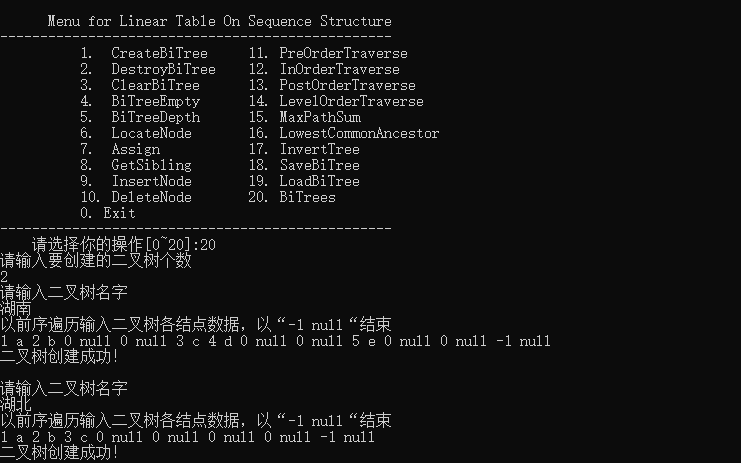
\includegraphics[width=16cm]{pic3//1.png}
    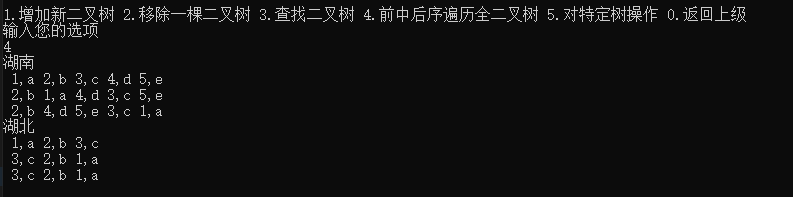
\includegraphics[width=16cm]{pic3//2.png}
    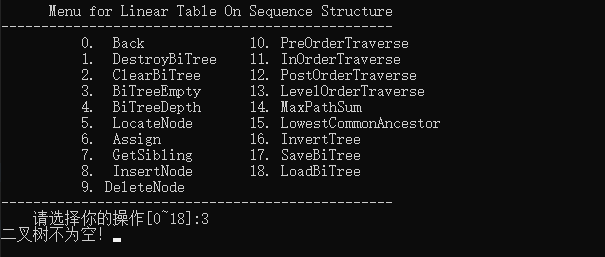
\includegraphics[width=16cm]{pic3//3.png}
    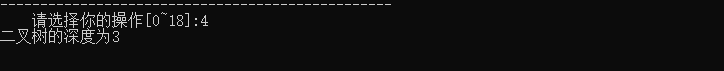
\includegraphics[width=16cm]{pic3//4.png}
\end{figure} 

\begin{figure}[H]
	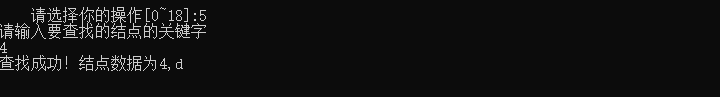
\includegraphics[width=16cm]{pic3//5.png}
	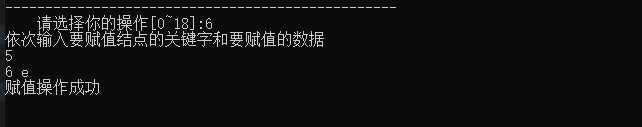
\includegraphics[width=16cm]{pic3//6.png}
	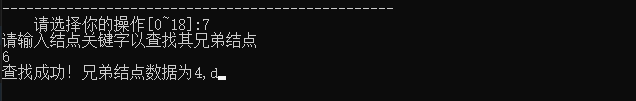
\includegraphics[width=16cm]{pic3//7.png}
	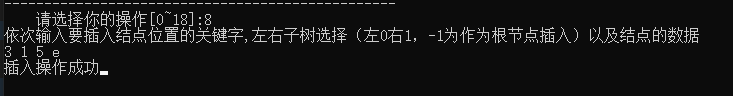
\includegraphics[width=16cm]{pic3//8.png}
	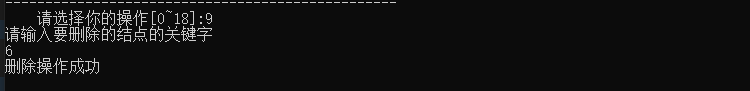
\includegraphics[width=16cm]{pic3//9.png}
	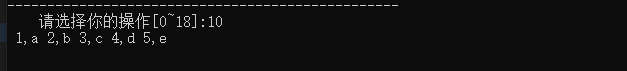
\includegraphics[width=16cm]{pic3//10.png}
	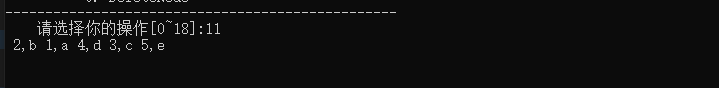
\includegraphics[width=16cm]{pic3//11.png}
	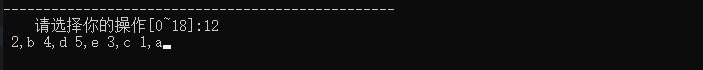
\includegraphics[width=16cm]{pic3//12.png}
	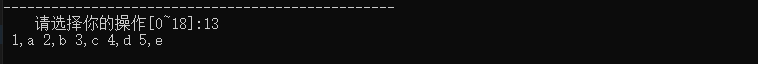
\includegraphics[width=16cm]{pic3//13.png}
	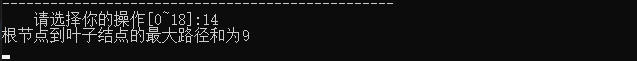
\includegraphics[width=16cm]{pic3//14.png}

\end{figure} 

\begin{figure}[H]
	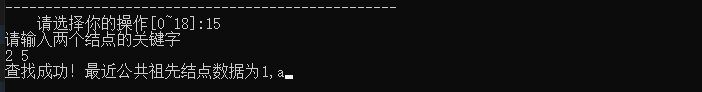
\includegraphics[width=16cm]{pic3//15.png}
	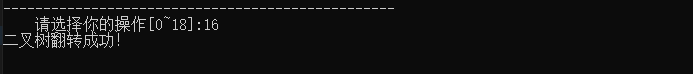
\includegraphics[width=16cm]{pic3//16.png}
	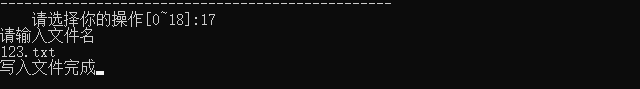
\includegraphics[width=16cm]{pic3//17.png}
	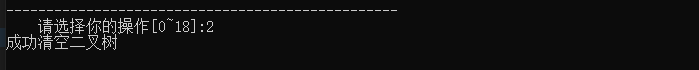
\includegraphics[width=16cm]{pic3//18.png}
	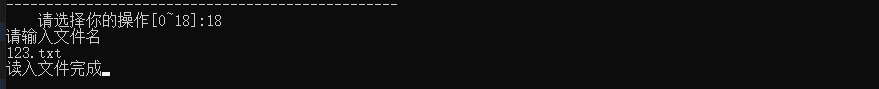
\includegraphics[width=16cm]{pic3//19.png}
	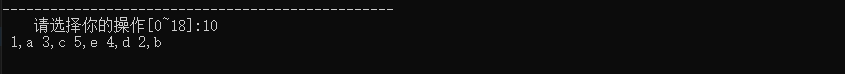
\includegraphics[width=16cm]{pic3//20.png}
\end{figure} 

\subsection{实验小结}
\begin{lstlisting}[breaklines][language=C]

本次实验的重难点有:
1.对指针的使用,要警惕和避免野指针的出现,容易访问非法内存导致程序出错。例如叶子节点指针域不为空;
2.对二叉树结构的熟练理解,确保对线性表执行的操作不产生错误或漏洞。例如节点的插入和删除;
3.对递归的使用,重在想要达到的效果而不是过程,要清楚地设置跳出递归的时机。
4.对栈和队列的使用。用于保存需要记录的数据。
4.多个二叉树管理表的设计和能够实现对每一个二叉树单独操作。
5.细节方面问题的处理:如,修改结点的值时,查无该结点和找到该结点但修改后的key发生了重复两种情况都应该说明清楚。
6.系统结构的设计,对使用进行合理的引导,令用户能够无需学习就上手,方便地使用功能;
本次实验的心得:
1.二叉树的结构相对于线性表更为复杂,同时涉及到了递归,栈和队列的使用,对知识和技能的掌握有更高的要求。
2.二叉树的插入和删除操作较为复杂,为了不造成数据的损失,需要对操作后的子树进行分类讨论和处理。
3.在做附加问题的最大路径和时,我还思考了从树中任意节点出发到任意节点的路径最大值,从而对dfs有了更加深度的理解。核心思想为递归地计算根节点左右子树的最大路径和,看是否大于0。伪代码如下:
int dfs(TreeNode root) {
        int max=0;
        if (root == NULL)
            return 0;
        int left_val = max(dfs(root->left), 0);
        int right_val = max(dfs(root->right), 0);
        max = max(root.val + left_val + right_val, max);
        return root.val + max(left_val, right_val);
    }
}
4.在做附加问题的最近公共祖先时,我不仅掌握了递归的查找方法,还掌握了用栈的方法。

\end{lstlisting}

\section{课程的收获和建议}

在本课程中,我学习了各种数据在计算机中的存储结构,理清了逻辑结构和物理结构的关系,掌握了对特定结构中存储的数据元素的各种操作,对计算机中数据的存储有了更加深刻的认识。

对本课程的建议是,希望能够有更多更方便地和老师交流与答疑的机会,能够在细节上查漏补缺。最后两个实验的时间稍显紧迫,可以适当调整课程开始时间。
学习了LaTeX的使用,真是受益匪浅呢(笑)。
\appendix
\section{附录 参考文献}
\begin{lstlisting}[breaklines][language=C]
[1]  卢萍,李开,王多强,甘早斌. C语言程序设计,北京:清华大学出版社,2019
[2]  [美]马克·艾伦·维斯. 数据结构与算法分析(C语言描述)第二版,机械工业出版社出版社
\end{lstlisting}


\end{sloppypar}
\end{document}